\section{Texteditoren}

\headlineframe{Texteditoren}

\headlineframe{Was haben die mit diesem Kurs zu tun?}

\begin{frame}{Texteditoren}
  \begin{itemize}
    \item Viele Dateien, denen man in der Wissenschaft begegnet, enthalten (plain) text
      \begin{itemize}
        \item Paper/Arbeiten mit \LaTeX
        \item Programm-Code
        \item Daten (csv, json, yaml, …)
        \item Emails
      \end{itemize}
    \item Es lohnt sich also, einen guten Texteditor zu wählen und den Umgang damit zu erlernen!
    \item Das spart auf lange Sicht Zeit und macht die Arbeit angenehmer
    \item Zwei Varianten: Terminal / GUI
  \end{itemize}
\end{frame}

\begin{frame}[c]{Textdateien und Unicode}
%    \textcolor{red}{Findet im SS24 schon die Data Literacy Veranstaltung statt?}
%    Dann können die nächsten beiden Folien raus.

  Was ist eigentlich eine Textdatei?

  \begin{itemize}
    \item In einer Datei stehen immer Binärdaten in Bytes, 1 Byte = 8 Bit, 0-255
    \item Es gibt (gab) viele Varianten, Text in Binärdaten umzuwandeln (Encoding)
    \item Heute sollte immer Unicode enkodiert als \texttt{utf-8} verwendet werden
    \item Es gibt viele standardisierte Dateiformate, die auf Textdateien basieren\\
      json, yaml, toml, ecsv, ...
    \item Und weniger standardisierte aber trotzdem verbreitete Formate: \\
      csv, fixed width table, ...
  \end{itemize}

  \begin{description}
    \item[Unicode]
      \begin{itemize}
        \item Sammlung von Schriftzeichen, Buchstaben, Akzente, Emojis, ...
        \item Aus allen Sprachen.
        \item Ordnet Zeichen \enquote{Codepoints} zu
        \item Beispiele: \texttt{LATIN SMALL LETTER A}: 97, \texttt{PILE OF POO}: 128169
      \end{itemize}
    \item[UTF-8] Encoding um Unicode-Text in Bytes zu speichern
  \end{description}
\end{frame}

\begin{frame}[c]{Zeilenende}

  Windows und Unix-Systeme verwenden unterschiedliche Konventionen für ein Zeilenende.

  \begin{description}
    \item[Unix] \mintinline{text}+\n+ \hspace{3.15em} \texttt{LF} (Linefeed)
    \item[Windows] \mintinline{text}+\r\n+ \hspace{2em} \texttt{CR LF} (Carriage Return + Linefeed).
  \end{description}

  VS Code/VS Codium erkennt auf allen Betriebssystemen, welche Konvention in der aktuellen Datei
  genutzt wird und behält sie bei.

  Empfehlung: immer Unix-Konvention nutzen

\end{frame}

\begin{frame}{Was muss ein Editor können?}
  \begin{minipage}{0.38\textwidth}
    In absteigender Wichtigkeit

    \begin{itemize}
      \item Zeilennummern
      \item Syntax-Highlighting
      \item Simple Autovervollständigung
      \item Plugins / Anpassbarkeit
      \item Linting (Warnhinweise für falschen Code)
      \item Komplexe Autovervollständigung (Snippets, Library-Funktionen)
    \end{itemize}
    
    \vspace{.4\textheight}
  \end{minipage}
  \pause
  \begin{minipage}{0.22\textwidth}
    Windows Notepad:

    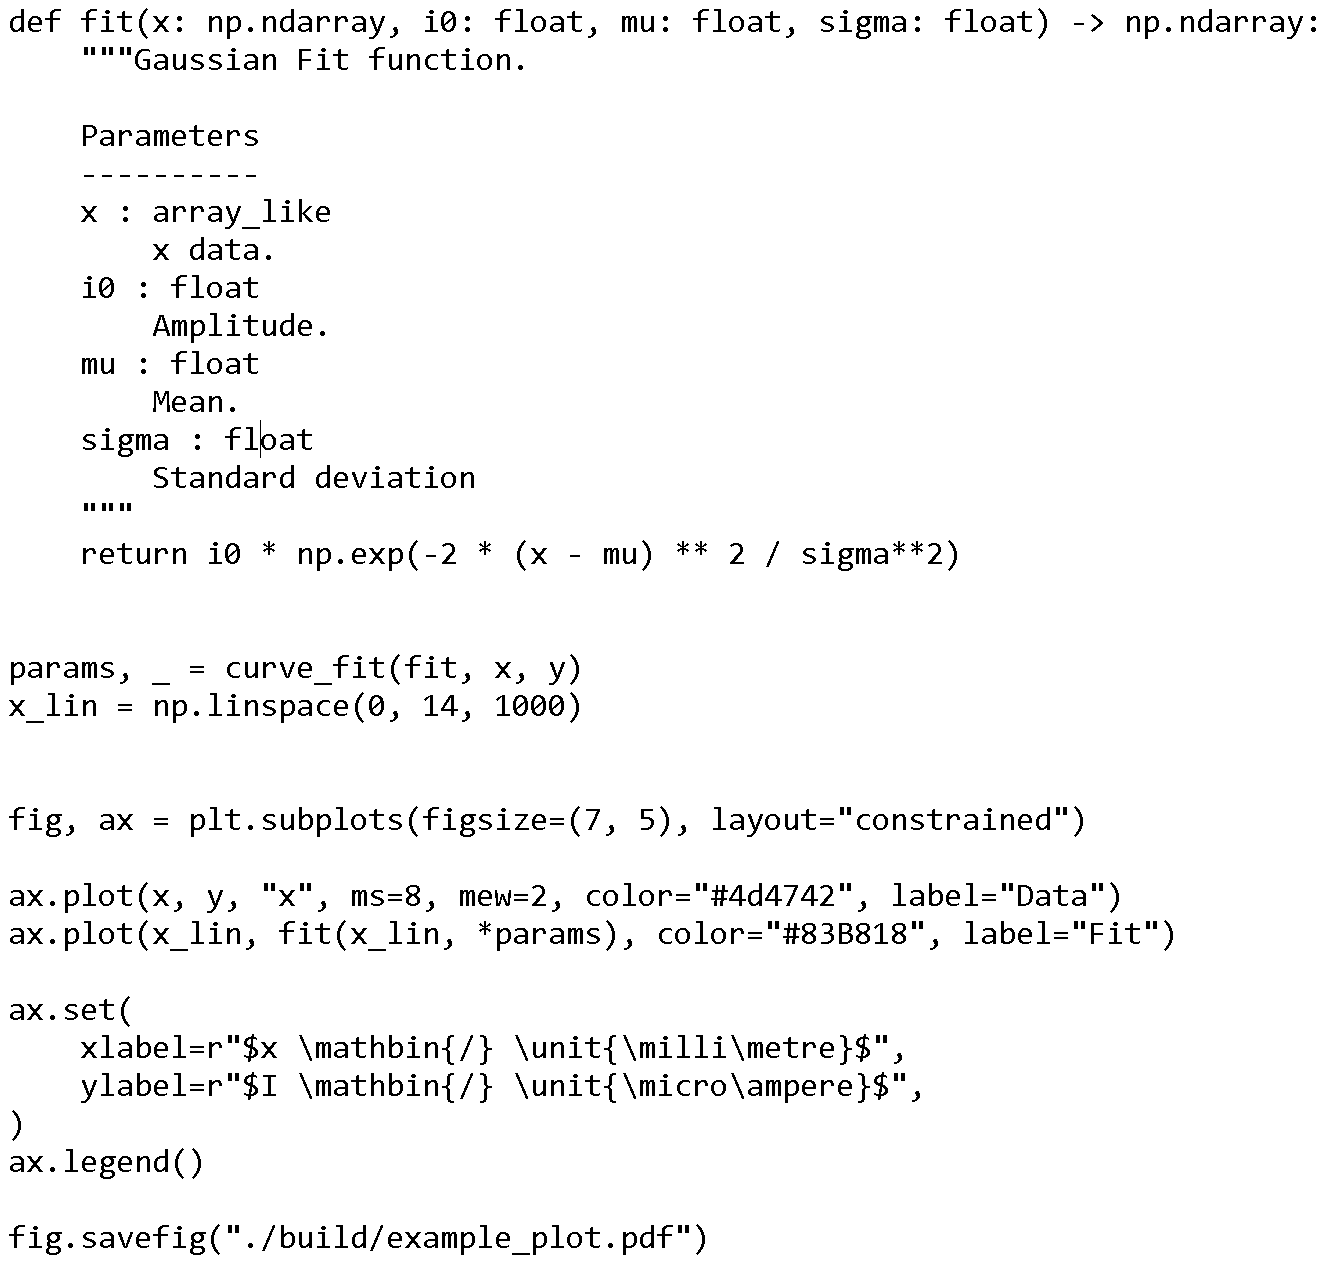
\includegraphics[height=0.52\textheight]{figures/notepad_example_screenshot.png}

    \vspace{.5\textheight}
  \end{minipage}
  \pause
  \begin{minipage}{0.3\textwidth}
    ~
    \vspace{.32\textheight}
    \flushright VS Codium: \flushleft \vspace{-1.5em}
    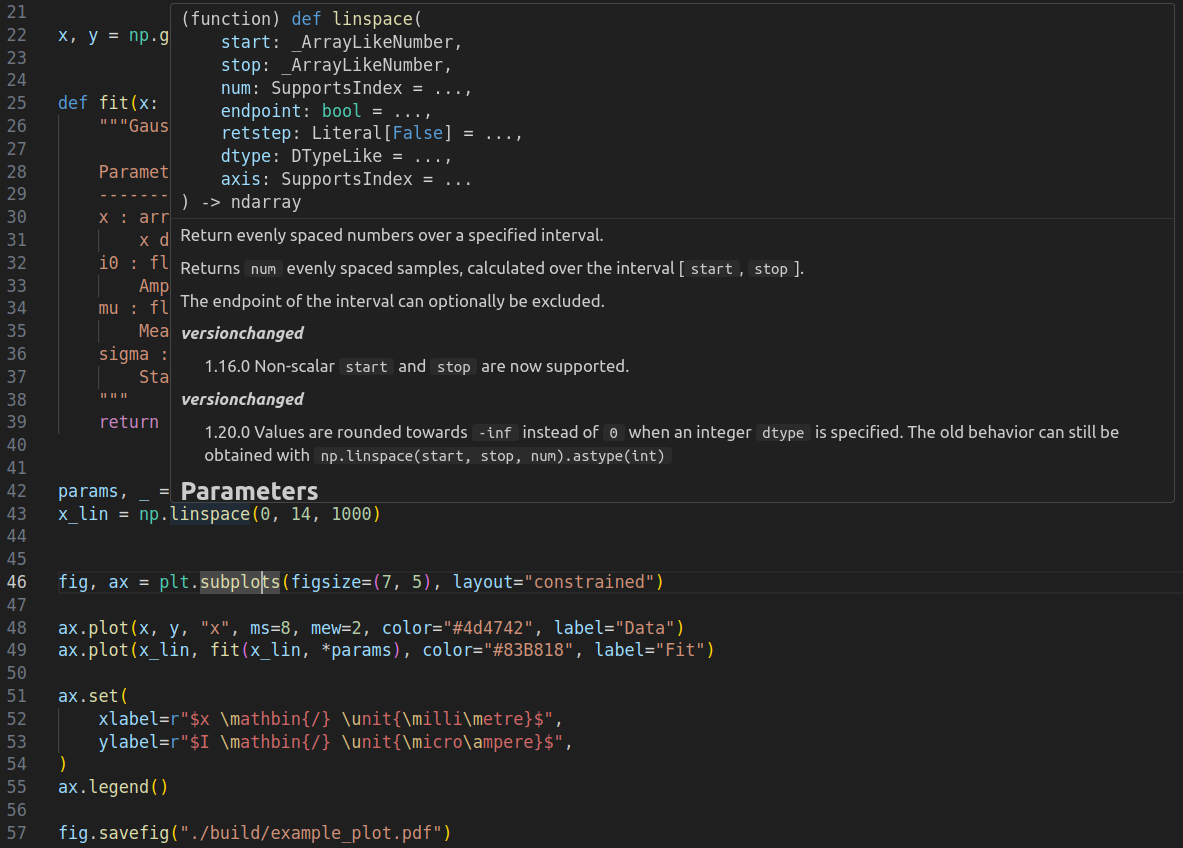
\includegraphics[height=0.52\textheight]{figures/vscodium_example_screenshot.png}
  \end{minipage}
\end{frame}

\begin{frame}{Nano, Vim, GUIs}
  \begin{tblr}{
      colspec = {X[c] X[c] X[c]},
      measure=vbox,
    }
    \textbf{\large Nano} & \textbf{\Large (Neo)Vim} & \textbf{\Large Visual Studio Code} \\
    \includegraphics[height=3cm]{figures/nano.png} &
    \includegraphics[height=3cm]{figures/vim.png} &
    \includegraphics[height=3cm]{figures/code.png} \\
    \begin{itemize}
      \item Einfacher Texteditor fürs Terminal
      \item Auf fast jedem Unix-System vorhanden
      \item Wenige Features, nicht erweiterbar
    \end{itemize}
    &
    \begin{itemize}
      \item Moden-basiert
      \item Erweiterbar
      \item Auf fast jedem Unix-System default
      \item Harter Einstieg
    \end{itemize}
    &
    \begin{itemize}
      \item GUI Editor von Microsoft
      \item Leichter zu bedienen
      \item Batteries included
      \item Viele nützliche Plugins
    \end{itemize}
    \\
  \end{tblr}
\end{frame}
